\newpage


\section*{Task 3}

Given a truth table, it was requested to see what happens
when the truth table is implemented with the smallest quantity of logic
gates. To perform this task, ICs that have NAND logic gates only
 will be used. This is because in most of ICs there are many
logic gates so it's a waste of logic gates if we use for example
just one of them. Note that this can also be implemented with 
NOR only ICs.

\subsection*{Low cost approach}
\begin{figure}[htbp]
    \begin{center}
    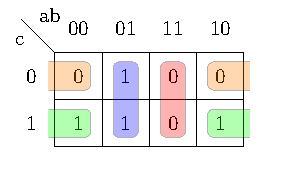
\includegraphics{data/karnaugh.pdf}
    
    \end{center}
    
    \caption{Karnaugh Map of the given truth table}
    \label{fig:KarnaughMap}
    \end{figure}
Let Z be the output label, its reduced minterms expression is:
\begin{equation}
    Z= (\bar{A}.B)+(C.\bar{B})
\end{equation} 
Also, its reduced maxterms expression is:
\begin{equation}
    Z= (\bar{A}+\bar{B}).(C+B)
\end{equation} 
\begin{figure}[htbp]
    \begin{center}
        \begin{tikzpicture}
            %seteamos el orden de las variables
            \node (x) at (0, 2)(x) {$A$};
            \node (y) at (0, 1) (y){$B$};
            \node (z) at (0, 0)(z) {$C$};
        
            %creamos un nodo con una posicion asociada:($(x)) que es donde se encuentra
            %posicionada la variable x y le ponemos nombre: nor_x
            %los numeros son para desplazar la compuertas
            \node[nor gate US, draw, rotate=0, logic gate inputs=nn] at ($(x) + (1.5, -0.075)$) (nor_x) {};
            \node[nor gate US, draw, rotate=0, logic gate inputs=nn] at ($(y) + (1.5, -0.075)$) (nor_y) {};
            
            %dibujar la nor con las entradas unidas:
            %primero dibujamos una linea
            \draw (x) -- (nor_x.input 1); 
            % ahora dibujamos desplazada la linea que va a entrar al input 2
            \draw (nor_x.input 2) -- ([xshift=-0.2cm]nor_x.input 2) |- (nor_x.input 1);
        
            \draw (y) -- (nor_y.input 1);
            \draw (nor_y.input 2) -- ([xshift=-0.2cm]nor_y.input 2) |- (nor_y.input 1);
        
            %asigno dos entradas
            \node[nor gate US, draw, rotate=0, logic gate inputs=nn] at ($(x) + (3, -0.075-0.5)$) (norAndB) {};
            \draw (nor_x.output) -- ([xshift=0.2cm]nor_x.output) |- (norAndB.input 1);
            \draw (nor_y.output) -- ([xshift=0.2cm]nor_y.output) |- (norAndB.input 2);
        
            \node[nor gate US, draw, rotate=0, logic gate inputs=nn] at ($(z) + (3, 0+0.10)$) (norBandC) {};
            \draw (z) -- ([xshift=0.2cm]z) |- (norBandC.input 2);
            \draw (y) -- ([xshift=-0.5cm]nor_y.input 1)  |- (norBandC.input 1);
        
            \node[nor gate US, draw, rotate=0, logic gate inputs=nn] at ($(y) + (4.5, -0.25)$) (norFinal) {};
            \draw (norAndB.output) -- ([xshift=0.2cm]norAndB.output) |- (norFinal.input 1);
            \draw (norBandC.output) -- ([xshift=0.2cm]norBandC.output) |- (norFinal.input 2);
        
            \draw (norFinal.output) -- node[above]{$Z$} ($(norFinal) + (1.5, 0)$);
        \end{tikzpicture}
        \begin{tikzpicture}
            \node (x) at (0, 2)(x) {$A$};
            \node (y) at (0, 1) (y){$B$};
            \node (z) at (0, 0)(z) {$C$};
            \node[nand gate US, draw, rotate=0, logic gate inputs=nn] at ($(x) + (1.5, -0.075)$) (nand_x) {};
            \draw (x) -- (nand_x.input 1); 
            \draw (nand_x.input 2) -- ([xshift=-0.2cm]nand_x.input 2) |- (nand_x.input 1);
            \draw (nand_x.output) -- node[right]{$N1$} ($(nand_x.output) + (0, 0)$);

            \node[nand gate US, draw, rotate=0, logic gate inputs=nn] at ($(x) + (3, -0.5)$) (nandAandB) {};
 


            \draw (nand_x.output) -- ([xshift=0.2cm]nand_x.output) |- (nandAandB.input 1) ;
            \node[nand gate US, draw, rotate=0, logic gate inputs=nn] at ($(y) + (1.5, -0.075)$) (nand_y) {};
            \draw (nand_y.output) -- node[right]{$N2$} ($(nand_y.output) + (0, 0)$);

            \draw (nandAandB.output) -- node[right]{$N3$} ($(nandAandB.output) + (0, 0)$);

            \draw (y) -- (nand_y.input 1); 
            \draw (nand_y.input 2) -- ([xshift=-0.2cm]nand_y.input 2) |- (nand_y.input 1);
            \draw (nand_y.input 1) -- ([yshift=0cm]nand_y.input 1) -- ([xshift=-0.5cm]nand_y.input 1) |- (nandAandB.input 2);
            \node[nand gate US, draw, rotate=0, logic gate inputs=nn] at ($(z) + (3,0.1)$) (nandBandC) {};
            
            \draw (nandBandC.output) -- node[right]{$N4$} ($(nandBandC) + (0.5, 0)$);
            
            \draw (z) -- (nandBandC.input 2); 
            \draw (nand_y.output) -- ([xshift=0.2cm]nand_y.output) |- (nandBandC.input 1);

            \node[nand gate US, draw, rotate=0, logic gate inputs=nn] at ($(y) + (5, -0.25)$) (nandFinal) {};
            \draw (nandAandB.output) -- ([xshift=0.2cm]nandAandB.output) |- (nandFinal.input 1);
            \draw (nandBandC.output) -- ([xshift=0.2cm]nandBandC.output) |- (nandFinal.input 2);
            \draw (nandFinal.output) -- node[above]{$Z$} ($(nandFinal) + (1.5, 0)$);

        \end{tikzpicture}



    \end{center}
    \caption{Implementation with NOR gates and NAND gates respectively}
\end{figure} 

Note that the quantity of logic gates in both cases are the same.

\section*{Hazards}

Sometimes propagation delays cause unexpected and unwanted transitions 
in the ouput. Depending on what we see in the output is how this issue is
called. If there is a transition from 1 to 0 and the output was supposed to
stay at 1 it is said that the circuit has a static 1-hazard. If the output must
go from 0 to 1(or 1 to 0) and before establishing at 1 (or 0), it changes its value 
it is said that the circuit has a dynamic hazard.

Hazards can always be found at the Karnaugh map.
An input that follows multiple paths to an output can create a glitch (due to the hazards in the circuit) if, for example, 
one path has an inverter (in this case implemented with a NAND logic gate) 
and one does not. This issue is called "asymmetric path delay" and it can be
seen in Figure~\ref{fig:KarnaughMap} with the input B. 

\begin{figure}[H] 
    \begin{center}
    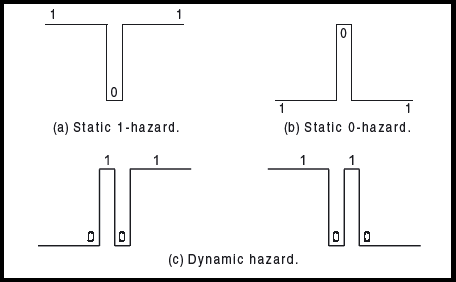
\includegraphics[width=0.45\textwidth]{data/hazard.png}
    \end{center}
    \caption{Different types of hazards}
    \label{fig:hazards}
    \end{figure} 



 \subsection*{Static 1-Hazard example} 
 Take the NAND implementation into account, assume all the propagation times 
 equal and then observe transition of the states A,B,C from 011 to 001 respectively.


\begin{figure}[H] 
    \begin{center}
    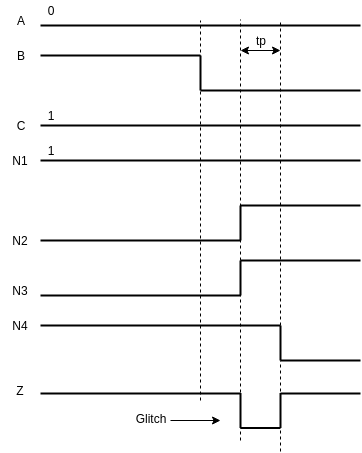
\includegraphics[width=6cm,height=8cm]{data/glitch.png}
    \end{center}
    \caption{Propagation time analysis}
    \label{fig:proptime}
    \end{figure} 
Note that tp in Figure~\ref{fig:proptime}  denotes the propagation time.

It can be seen that there should be a glitch at the output.The different combination of delays that produce a glitch may or may not be likely 
to occur in the implementation of the circuit. In some instances it is very 
unlikely that such delays would occur.


\section*{Measures obtained from NAND implementation}
\begin{figure}[H] 
\begin{center}
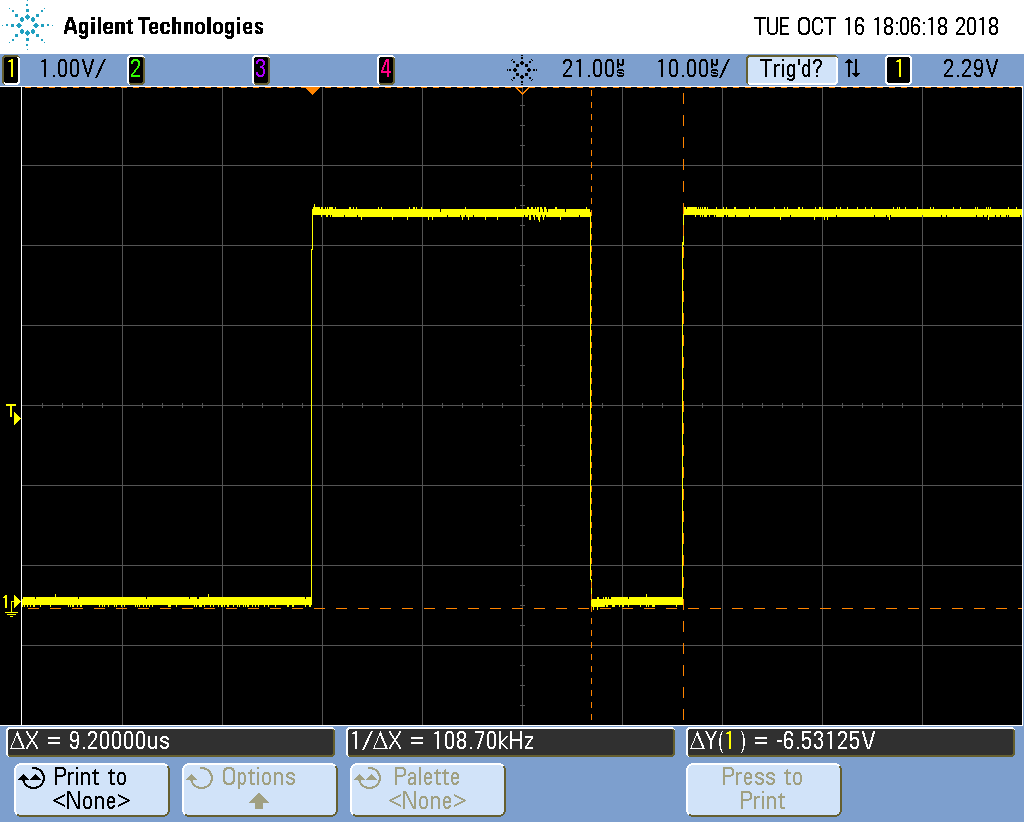
\includegraphics[width=0.45\textwidth]{data/000to001.png}
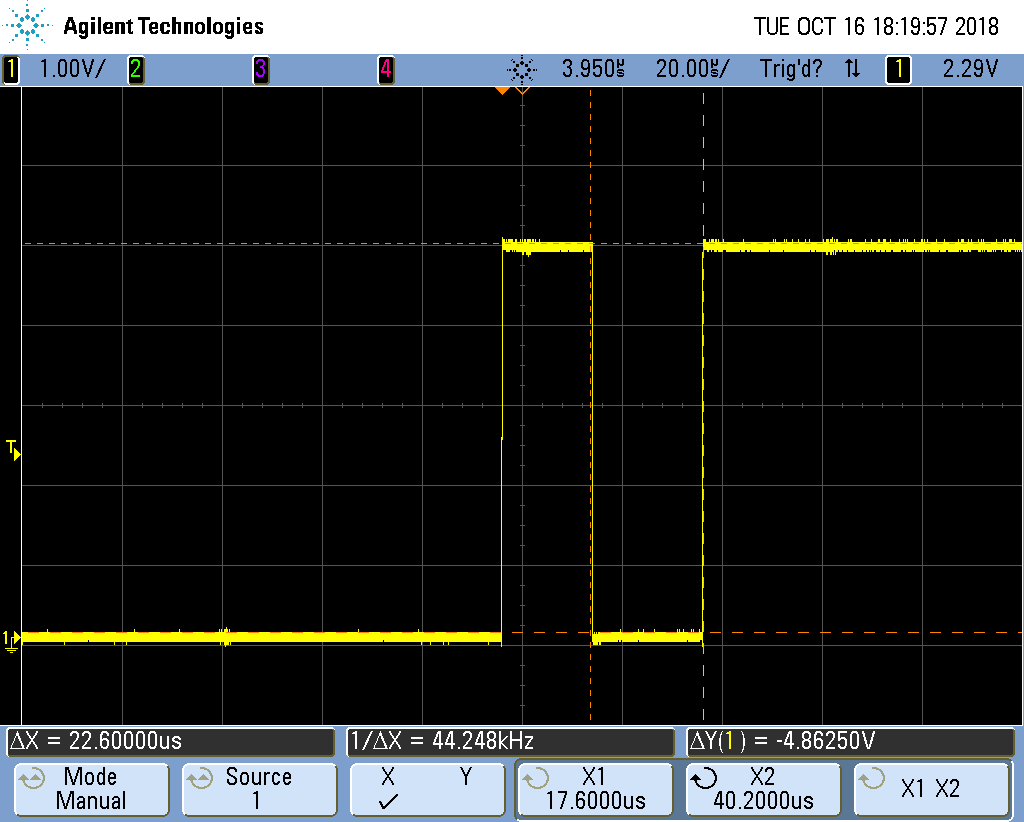
\includegraphics[width=0.45\textwidth]{data/000to001_11.png}
\end{center}
\caption{Dynamic hazards}
\label{fig:measure_dynamic}
\end{figure} 
In order to get the measures it was required to trigger many times until one of these 
glitches appear. It can be seen in Figure~\ref{fig:measure_dynamic} that glitches caused by dynamic hazards doesn't share the same time interval in spite of being the same transition
(from 000 to 001), this gives us some idea of delay propagation. 

\begin{figure}[H] 
\begin{center}
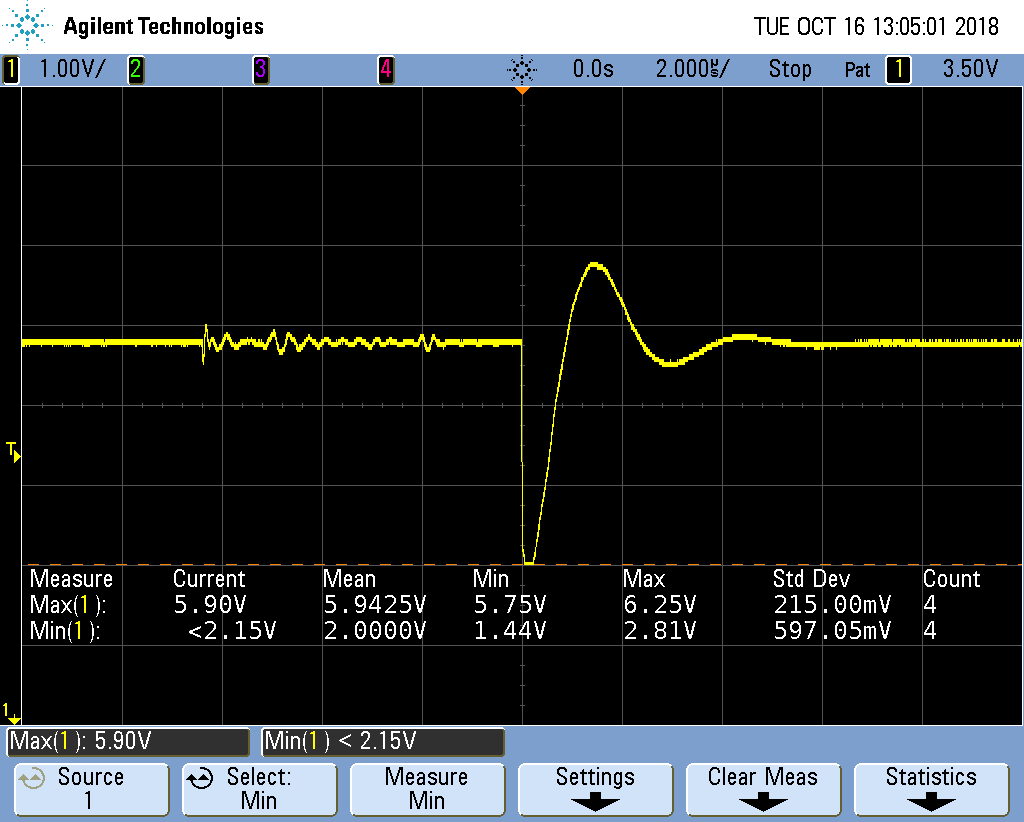
\includegraphics[width=0.45\textwidth]{data/001to011.png}
\end{center}
\caption{Static 1-hazard}
\label{fig:measure_static}
\end{figure} 
The measure in Figure~\ref{fig:measure_static} was made with the transition 001 to 011 and the
 trigger configured to get the negative-edge so these glitches can be found.


\section*{Conclusion}
In order to remove glitches it is needed to add redundant groups in the
Karnaugh Map so that disjoint groups overlap.
\begin{figure}[H] 
    \begin{center}
    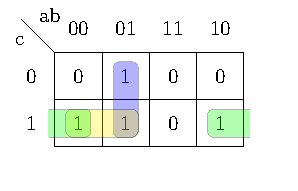
\includegraphics{data/karnaugh_improved.pdf}
    \end{center}
    \caption{Karnaugh with redundant logic}
    \label{fig:karnaugh_improved}
    \end{figure} 
In this case the output is given by:
\begin{equation*}
    Z= (\bar{A}+\bar{B}).(C+B)+(\bar{A}.C)    
\end{equation*} 

Note that the new term term of the expression is not dependent
of B so regardless of the variation of B there won't be glitches
in the output.

